%%%%%%%%%%%%%%%%%%%%%%%%%%%%%%%%%%%%%%%%%%%%%%%%%%%%%%%%%%%%
%%  This Beamer template was created by Cameron Bracken.
%%  Anyone can freely use or modify it for any purpose
%%  without attribution.
%%
%%  Last Modified: January 9, 2009
%%
%%
%%
%% notes: 
%% This document compiles very easily using the
%% LaTeX Tools or LaTeXing packages of Sublime Text.
%%

\documentclass[xcolor=x11names,compress]{beamer}

%%%%%%%%%%%%%%%%%%%%%%%%%%%%%%%%%%%%%%%%%%%%%%%%%%%%%%
%% General document
%%%%%%%%%%%%%%%%%%%%%%%%%%%%%%%%%%%%%%%%%%%%%%%%%%%%%%
\usepackage{graphicx}
\usepackage{tikz}
\usetikzlibrary{decorations.fractals}
\usepackage{color}
\usepackage{listings}
\lstset{ %
		language=[LaTeX]TeX,
		basicstyle=\normalsize\ttfamily,
		keywordstyle=,
		numbers=left,
		numberstyle=\tiny\ttfamily,
		stepnumber=1,
		showspaces=false,
		showstringspaces=false,
		showtabs=false,
		breaklines=true,
		frame=tb,
		framerule=0.5pt,
		tabsize=4,
		framexleftmargin=0.5em,
		framexrightmargin=0.5em,
		xleftmargin=0.5em,
		xrightmargin=0.5em
		}

% \usepackage{multicol}
% \renewcommand{\(}{\begin{columns}}
% \renewcommand{\)}{\end{columns}}
% \newcommand{\<}[1]{\begin{column}{#1}}
% \renewcommand{\>}{\end{column}}


%%%%%%%%%%%%%%%%%%%%%%%%%%%%%%%%%%%%%%%%%%%%%%%%%%%%%%
%% Beamer Layout 
%%%%%%%%%%%%%%%%%%%%%%%%%%%%%%%%%%%%%%%%%%%%%%%%%%%%%%
\useoutertheme[subsection=false,shadow]{miniframes}


%% A simple footer only with page-number
\setbeamertemplate{footline}[page number]
\setbeamertemplate{navigation symbols}{}%remove navigation symbols
\useinnertheme{default}
\usefonttheme{serif}
\usepackage{palatino}
\setbeamerfont{title like}{shape=\scshape}
\setbeamerfont{frametitle}{shape=\scshape}
\setbeamercolor*{lower separation line head}{bg=DeepSkyBlue4} 
\setbeamercolor*{normal text}{fg=black,bg=white} 
\setbeamercolor*{alerted text}{fg=red} 
\setbeamercolor*{example text}{fg=black} 
\setbeamercolor*{structure}{fg=black} 
\setbeamercolor*{palette tertiary}{fg=black,bg=black!10} 
\setbeamercolor*{palette quaternary}{fg=black,bg=black!10} 


%%%%%%%%%%%%%%%%%%%%%%%%%%%%%%%%%%%%%%%%%%%%%%%%%%%%%%
%% Citations and Bibliography styles
%%%%%%%%%%%%%%%%%%%%%%%%%%%%%%%%%%%%%%%%%%%%%%%%%%%%%%
\usepackage[backend=bibtex,
			style=ieee,
			natbib=true,
			firstinits=true,
			maxnames=99,
			volume=false,
			number=false,
			pages=false,
			doi=false,
			url=false,
			issn=false]
			{biblatex}

\addbibresource{fastFlume.bib}
\renewcommand*{\bibfont}{\footnotesize}
% \\renewcommand*{\bibfont}{\footnotesize}
% {\footnotesize\bibliography{fastFlume.bib}}

\setbeamertemplate{bibliography item}[text]

\newcommand{\customcite}[1]{\citeauthor{#1}, \citetitle{#1}, \citeyear{#1}}
\newcommand{\customfootcite}[1]{\footnote{\citeauthor{#1}, \citetitle{#1}, \citeyear{#1}}}

\setbeamerfont{footnote}{size=\tiny}

%%%%%%%%%%%%%%%%%%%%%%%%%%%%%%%%%%%%%%%%%%%%%%%%%%%%%%
%%%%%%%%%%%%%%%%%%%%%%%%%%%%%%%%%%%%%%%%%%%%%%%%%%%%%%
%%%%%%%%%%%%%%%%%%%%%%%%%%%%%%%%%%%%%%%%%%%%%%%%%%%%%%
%%%%%%%%%%%%%%%%%%%%%%%%%%%%%%%%%%%%%%%%%%%%%%%%%%%%%%
%%%%%%%%%%%%%%%%%%%%%%%%%%%%%%%%%%%%%%%%%%%%%%%%%%%%%%
%%%%%%%%%%%%%%%%%%%%%%%%%%%%%%%%%%%%%%%%%%%%%%%%%%%%%%
%%%%%%%%%%%%%%%%%%%%%%%%%%%%%%%%%%%%%%%%%%%%%%%%%%%%%%
%%%%%%%%%%%%%%%%%%%%%%%%%%%%%%%%%%%%%%%%%%%%%%%%%%%%%%
%%%%%%%%%%%%%%%%%%%%%%%%%%%%%%%%%%%%%%%%%%%%%%%%%%%%%%
%%%%%%%%%%%%%%%%%%%%%%%%%%%%%%%%%%%%%%%%%%%%%%%%%%%%%%

\title{Study of Hydrokinetic Turbine Arrays with Large Eddy Simulation}
\subtitle{\small "fastFlume" tutorial for SOWFA}

\author{Danny Clay Sale (dsale@uw.edu)}

\institute{\small University of Washington, Seattle, WA, USA\\
           Department of Mechanical Engineering\\
           Northwest National Marine Renewable Energy Center}
           
%%%%%%%%%%%%%%%%%%%%%%%%%%%%%%%%%%%%%%%%%%%%%%%%%%%%%%
%% Main body of document
%%%%%%%%%%%%%%%%%%%%%%%%%%%%%%%%%%%%%%%%%%%%%%%%%%%%%%
\begin{document}


%%%%%%%%%%%%%%%%%%%%%%%%%%%%%%%%%%%%%%%%%%%%%%%%%%%%%%
%%%%%%%%%%%%%%%%%%%%%%%%%%%%%%%%%%%%%%%%%%%%%%%%%%%%%%
%%%%%%%%%%%%%%%%%%%%%%%%%%%%%%%%%%%%%%%%%%%%%%%%%%%%%%
%%%%%%%%%%%%%%%%%%%%%%%%%%%%%%%%%%%%%%%%%%%%%%%%%%%%%%
%%%%%%%%%%%%%%%%%%%%%%%%%%%%%%%%%%%%%%%%%%%%%%%%%%%%%%
%%%%%%%%%%%%%%%%%%%%%%%%%%%%%%%%%%%%%%%%%%%%%%%%%%%%%%
%%%%%%%%%%%%%%%%%%%%%%%%%%%%%%%%%%%%%%%%%%%%%%%%%%%%%%
%%%%%%%%%%%%%%%%%%%%%%%%%%%%%%%%%%%%%%%%%%%%%%%%%%%%%%
%%%%%%%%%%%%%%%%%%%%%%%%%%%%%%%%%%%%%%%%%%%%%%%%%%%%%%
%%%%%%%%%%%%%%%%%%%%%%%%%%%%%%%%%%%%%%%%%%%%%%%%%%%%%%
\section{\scshape Intro}

	\subsection{titlepage}
			\begin{frame}
				\titlepage
			\end{frame}

	\subsection{Focus}
		\begin{frame}{Focus}

			What is the potential power generation and environmental effects from marine hydro-kinetic (MHK) turbine farms?

			\begin{itemize}
				\item Areas to Investigate
					\begin{itemize}
						\item fluctuations of power production and structural response due to turbulence
						\item turbulence characteristics and wake evolution
						\item near field pressure fluctuations in wake
					\end{itemize}

				\item Comparison of Numerical Simulations and Experiment
					\begin{itemize}
						\item physical testing of 3 turbines in water flume
						\item large-eddy-simulation (LES) to replicate experiment
					\end{itemize}

			\end{itemize}

		\end{frame}

%%%%%%%%%%%%%%%%%%%%%%%%%%%%%%%%%%%%%%%%%%%%%%%%%%%%%%
%%%%%%%%%%%%%%%%%%%%%%%%%%%%%%%%%%%%%%%%%%%%%%%%%%%%%%
%%%%%%%%%%%%%%%%%%%%%%%%%%%%%%%%%%%%%%%%%%%%%%%%%%%%%%
%%%%%%%%%%%%%%%%%%%%%%%%%%%%%%%%%%%%%%%%%%%%%%%%%%%%%%
%%%%%%%%%%%%%%%%%%%%%%%%%%%%%%%%%%%%%%%%%%%%%%%%%%%%%%
%%%%%%%%%%%%%%%%%%%%%%%%%%%%%%%%%%%%%%%%%%%%%%%%%%%%%%
%%%%%%%%%%%%%%%%%%%%%%%%%%%%%%%%%%%%%%%%%%%%%%%%%%%%%%
%%%%%%%%%%%%%%%%%%%%%%%%%%%%%%%%%%%%%%%%%%%%%%%%%%%%%%
%%%%%%%%%%%%%%%%%%%%%%%%%%%%%%%%%%%%%%%%%%%%%%%%%%%%%%
%%%%%%%%%%%%%%%%%%%%%%%%%%%%%%%%%%%%%%%%%%%%%%%%%%%%%%
\section{\scshape Experiment}

	\subsection{Flume and Turbines}

	\begin{frame}{Tidal Turbine Reference Model 1}

		\begin{columns}
		    
		    \begin{column}{0.45\textwidth}
		        % \rule{\textwidth}{0.75\textwidth}

		        \begin{figure}[p]
				    \centering
				    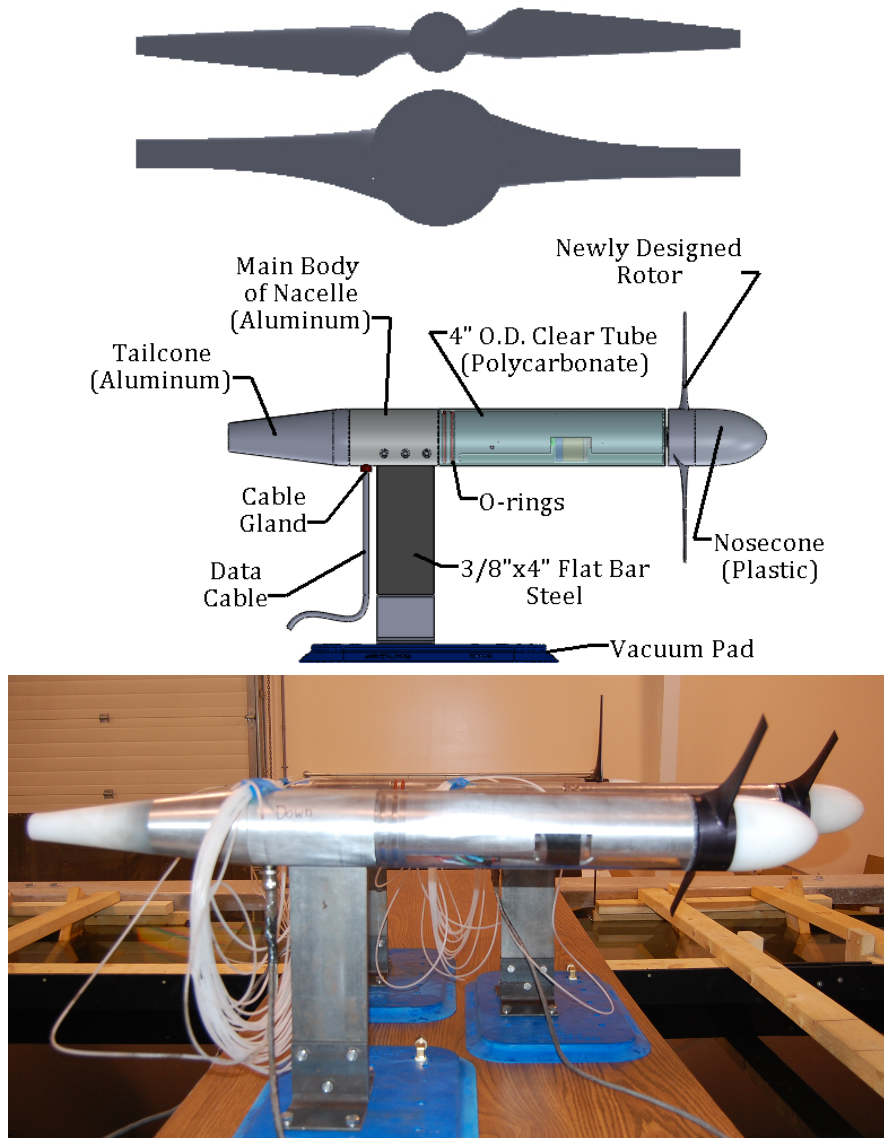
\includegraphics[width=1.1\textwidth]{figures/Nicks_turbines_redesign.png}
				\end{figure}

		    \end{column}
		    
		    \begin{column}{0.55\textwidth}
				
				\begin{itemize}
					\item \footnotesize horizontal-axis turbine, full-scale 550kW, diameter of 20-m
					\item created by US DOE to standardize experimental and numerical studies
					\item foils are NACA 4 and 6 series chosen for cavitation prevention and well known performance characteristics at low and high Reynolds
					\item laboratory turbine 45:1 scaling -- diameter of 45-cm
					\item attempt to match power extraction and wake characteristics at lab-scale
					\item lab-scale rotor was re-designed to minimize Reynolds scaling effects
				\end{itemize}
		    
		    \end{column}

		\end{columns}

	\end{frame}



	\begin{frame}{Flume Testing of 3 Turbines}

		\begin{figure}[p]
		    \centering
		    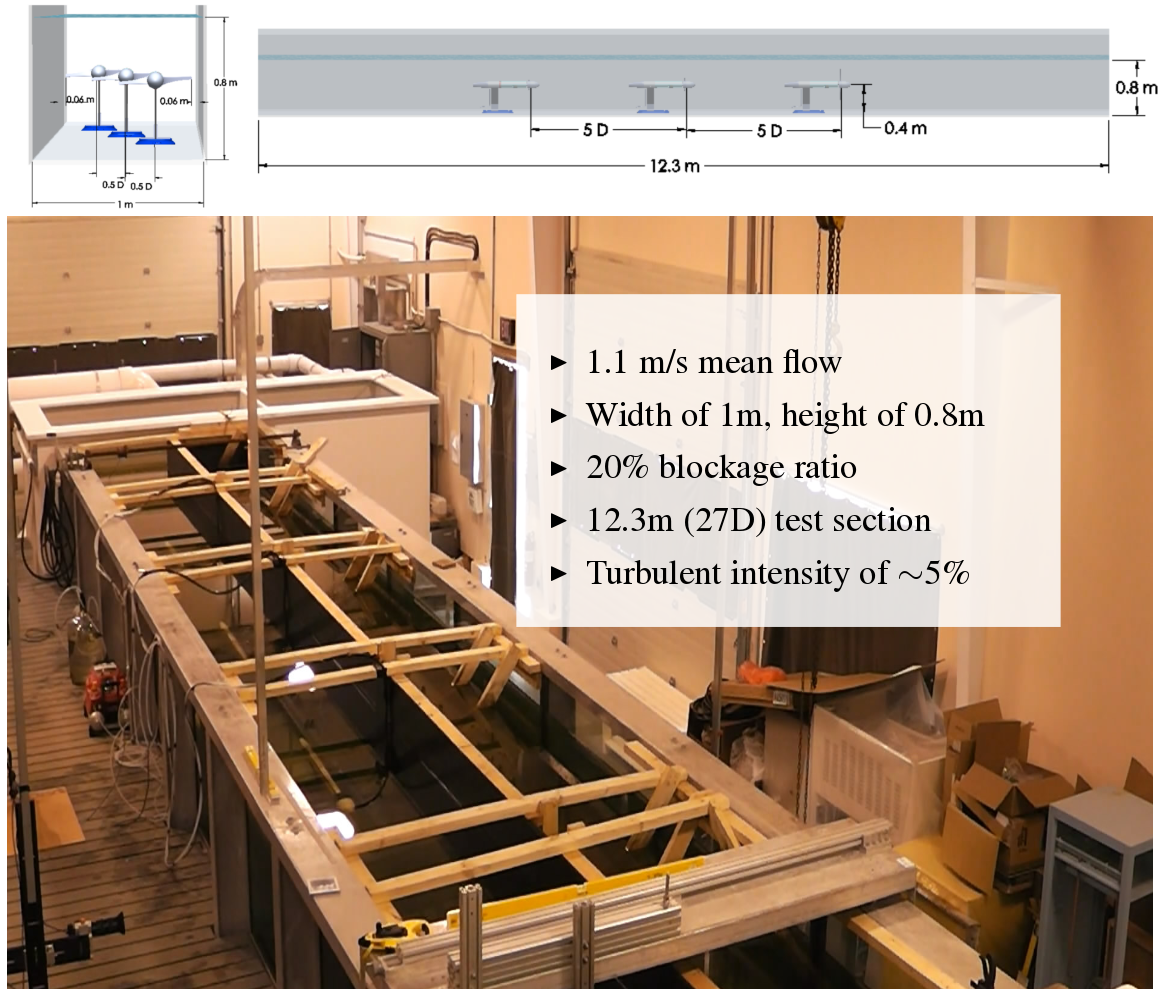
\includegraphics[width=1.0\textwidth]{figures/flume_and_description_v2.png}
		\end{figure}


	\end{frame}

	\begin{frame}{Visualization of Tip Vortex}

		\begin{figure}[p]
		    \item bubbles are released from the nacelle to visualize tip vortex (movie)
		    \centering
		    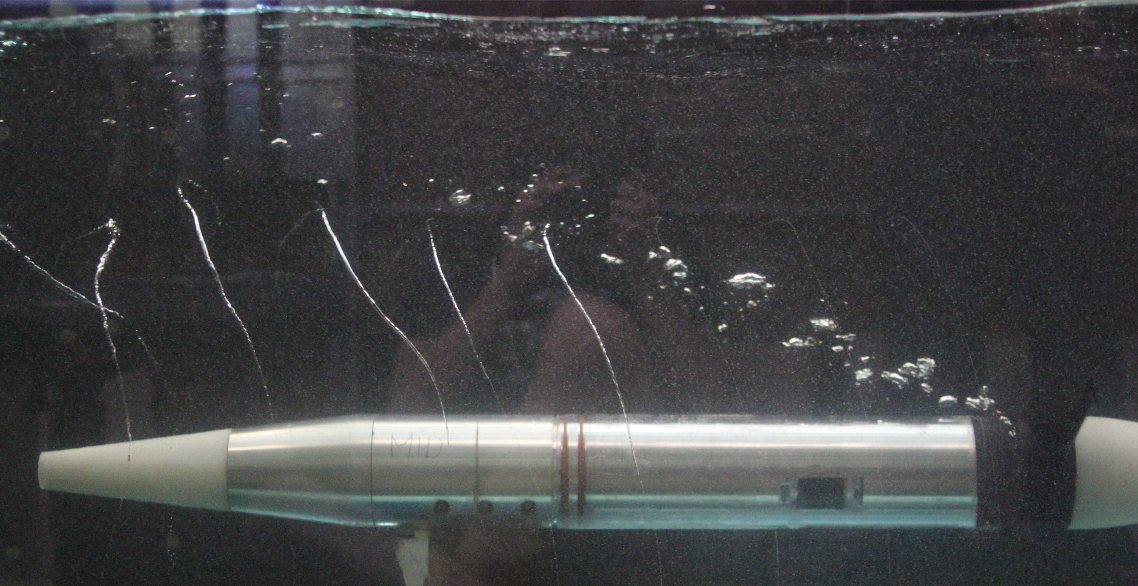
\includegraphics[width=1.0\textwidth]{figures/turbine_tip_vortex_and_bubbles.png}
		\end{figure}


	\end{frame}

%%%%%%%%%%%%%%%%%%%%%%%%%%%%%%%%%%%%%%%%%%%%%%%%%%%%%%
%%%%%%%%%%%%%%%%%%%%%%%%%%%%%%%%%%%%%%%%%%%%%%%%%%%%%%
%%%%%%%%%%%%%%%%%%%%%%%%%%%%%%%%%%%%%%%%%%%%%%%%%%%%%%
%%%%%%%%%%%%%%%%%%%%%%%%%%%%%%%%%%%%%%%%%%%%%%%%%%%%%%
%%%%%%%%%%%%%%%%%%%%%%%%%%%%%%%%%%%%%%%%%%%%%%%%%%%%%%
%%%%%%%%%%%%%%%%%%%%%%%%%%%%%%%%%%%%%%%%%%%%%%%%%%%%%%
%%%%%%%%%%%%%%%%%%%%%%%%%%%%%%%%%%%%%%%%%%%%%%%%%%%%%%
%%%%%%%%%%%%%%%%%%%%%%%%%%%%%%%%%%%%%%%%%%%%%%%%%%%%%%
%%%%%%%%%%%%%%%%%%%%%%%%%%%%%%%%%%%%%%%%%%%%%%%%%%%%%%
%%%%%%%%%%%%%%%%%%%%%%%%%%%%%%%%%%%%%%%%%%%%%%%%%%%%%%
\section{\scshape Numerical Model}

\subsection{LES and ALM}
\begin{frame}{}

\small The turbine model uses the 
velocity field from the LES to compute the 
hydrodynamic forces imparted on the turbine blades, and
then body forces are projected back onto flow field.
\footfullcite{SOWFA_a}

\vspace{-10pt}

\begin{columns}
		    
    \begin{column}{0.3\textwidth}
        % \rule{\textwidth}{0.75\textwidth}

\vspace{-10pt}

        \begin{figure}[p]
		    \centering
		    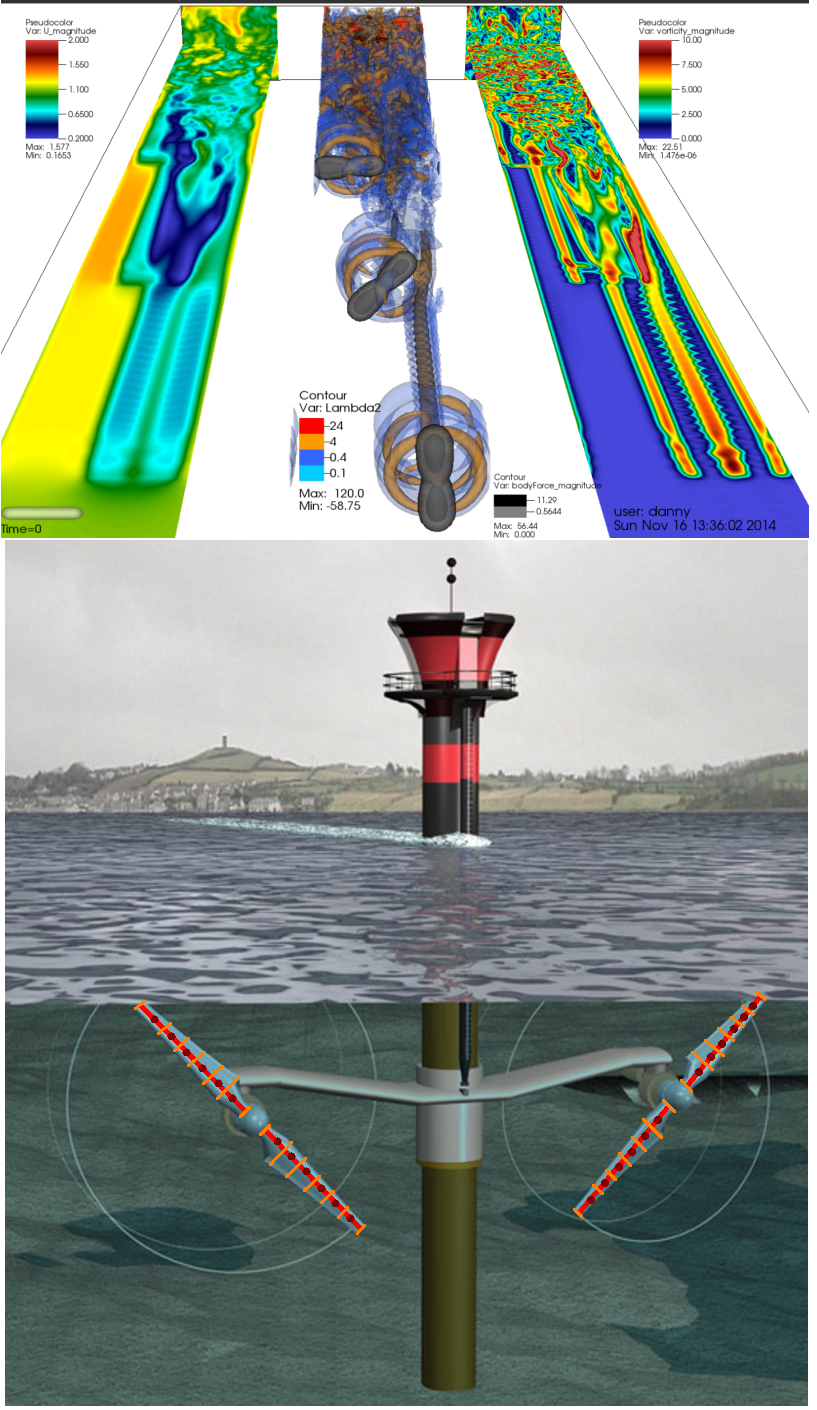
\includegraphics[width=1.1\textwidth]{figures/LES_and_cartoon_actuator_line.png}
		\end{figure}

    \end{column}
    
    \begin{column}{0.875\textwidth}
		
		\begin{itemize}
			\item \small Large-Eddy-Simulation (LES)
			\vspace{-5pt}
				\begin{itemize}
					\item \small code: OpenFOAM (\scriptsize{Field Operation and Manipulation})
					\item second-order accurate finite-volume (FV) formulation 
					\item filter is implicitly defined by the mesh and FV discretization
					\item subgrid-stress (SGS) model is constant coefficient Smagorinsky
				\end{itemize}

			\item Actuator-Line-Method (ALM)
			\vspace{-5pt}
				\begin{itemize}
					\item \small code: FAST (\scriptsize{Fatigue Aerodynamics Structures Turbulence})
					\item creates turbulent wake and captures blade tip and root vortices
					\item similar to blade element method discretize blades into spanwise sections
					\item depends on airfoil lookup tables for lift, drag, moment, min. pressure coefficients
					\item normalized forces projected onto flow field with equal and opposite direction
				\end{itemize}

		\end{itemize}
    
    \end{column}

\end{columns}



\end{frame}



%%%%%%%%%%%%%%%%%%%%%%%%%%%%%%%%%%%%%%%%%%%%%%%%%%%%%%
%%%%%%%%%%%%%%%%%%%%%%%%%%%%%%%%%%%%%%%%%%%%%%%%%%%%%%
%%%%%%%%%%%%%%%%%%%%%%%%%%%%%%%%%%%%%%%%%%%%%%%%%%%%%%
%%%%%%%%%%%%%%%%%%%%%%%%%%%%%%%%%%%%%%%%%%%%%%%%%%%%%%
%%%%%%%%%%%%%%%%%%%%%%%%%%%%%%%%%%%%%%%%%%%%%%%%%%%%%%
%%%%%%%%%%%%%%%%%%%%%%%%%%%%%%%%%%%%%%%%%%%%%%%%%%%%%%
%%%%%%%%%%%%%%%%%%%%%%%%%%%%%%%%%%%%%%%%%%%%%%%%%%%%%%
%%%%%%%%%%%%%%%%%%%%%%%%%%%%%%%%%%%%%%%%%%%%%%%%%%%%%%
%%%%%%%%%%%%%%%%%%%%%%%%%%%%%%%%%%%%%%%%%%%%%%%%%%%%%%
%%%%%%%%%%%%%%%%%%%%%%%%%%%%%%%%%%%%%%%%%%%%%%%%%%%%%%

\section{\scshape Simulation Lab Scale}

\subsection{3 turbines}

	\begin{frame}{Turbines=3  TSR=6.2  Mesh=(coarse, medium)}
		
		\begin{columns}
		    
		    \begin{column}{0.6\textwidth}
		        \begin{figure}[p]
				    \centering
				    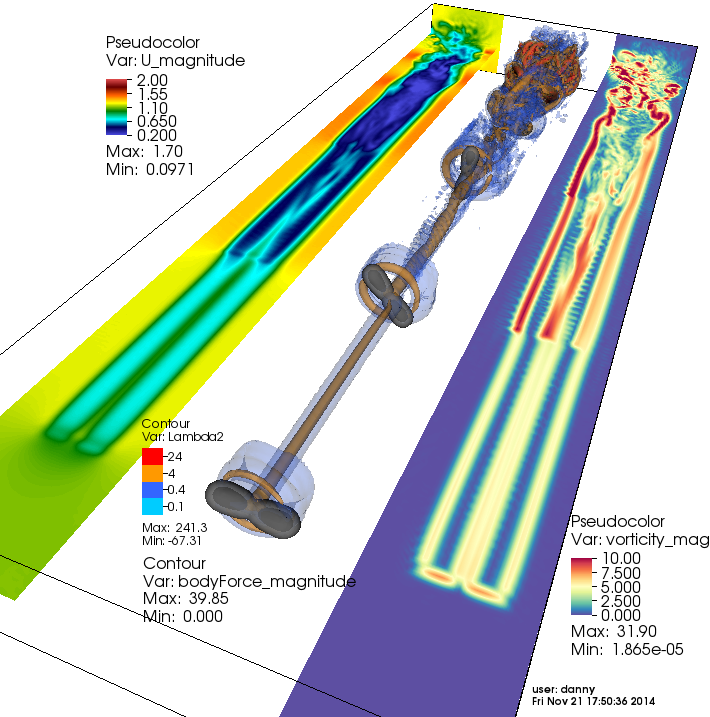
\includegraphics[width=0.8\textwidth]{figures/fastFlume__Turbines=3_TSR=6p2_Layout=offset_Mesh=coarse.png}
				    \caption{\scriptsize{coarse mesh 465x50x40, dx = 0.020 m}}
				\end{figure}

		    \end{column}
		    
		    \begin{column}{0.6\textwidth}
		        \begin{figure}[p]
				    \centering
				    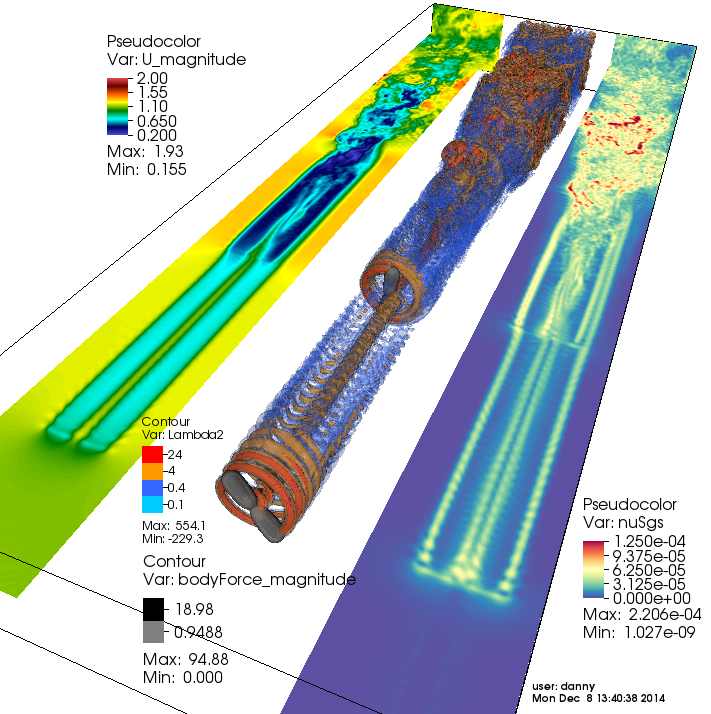
\includegraphics[width=0.8\textwidth]{figures/fastFlume__Turbines=3_TSR=6p2_Layout=offset_Mesh=medium.png}
				    \caption{\scriptsize{medium mesh 698x75x60, dx = 0.013 m}}
				\end{figure}

		    \end{column}

		\end{columns}

	\end{frame}


	\begin{frame}{at higher resolution}

		\begin{figure}[p]
		    \centering
    		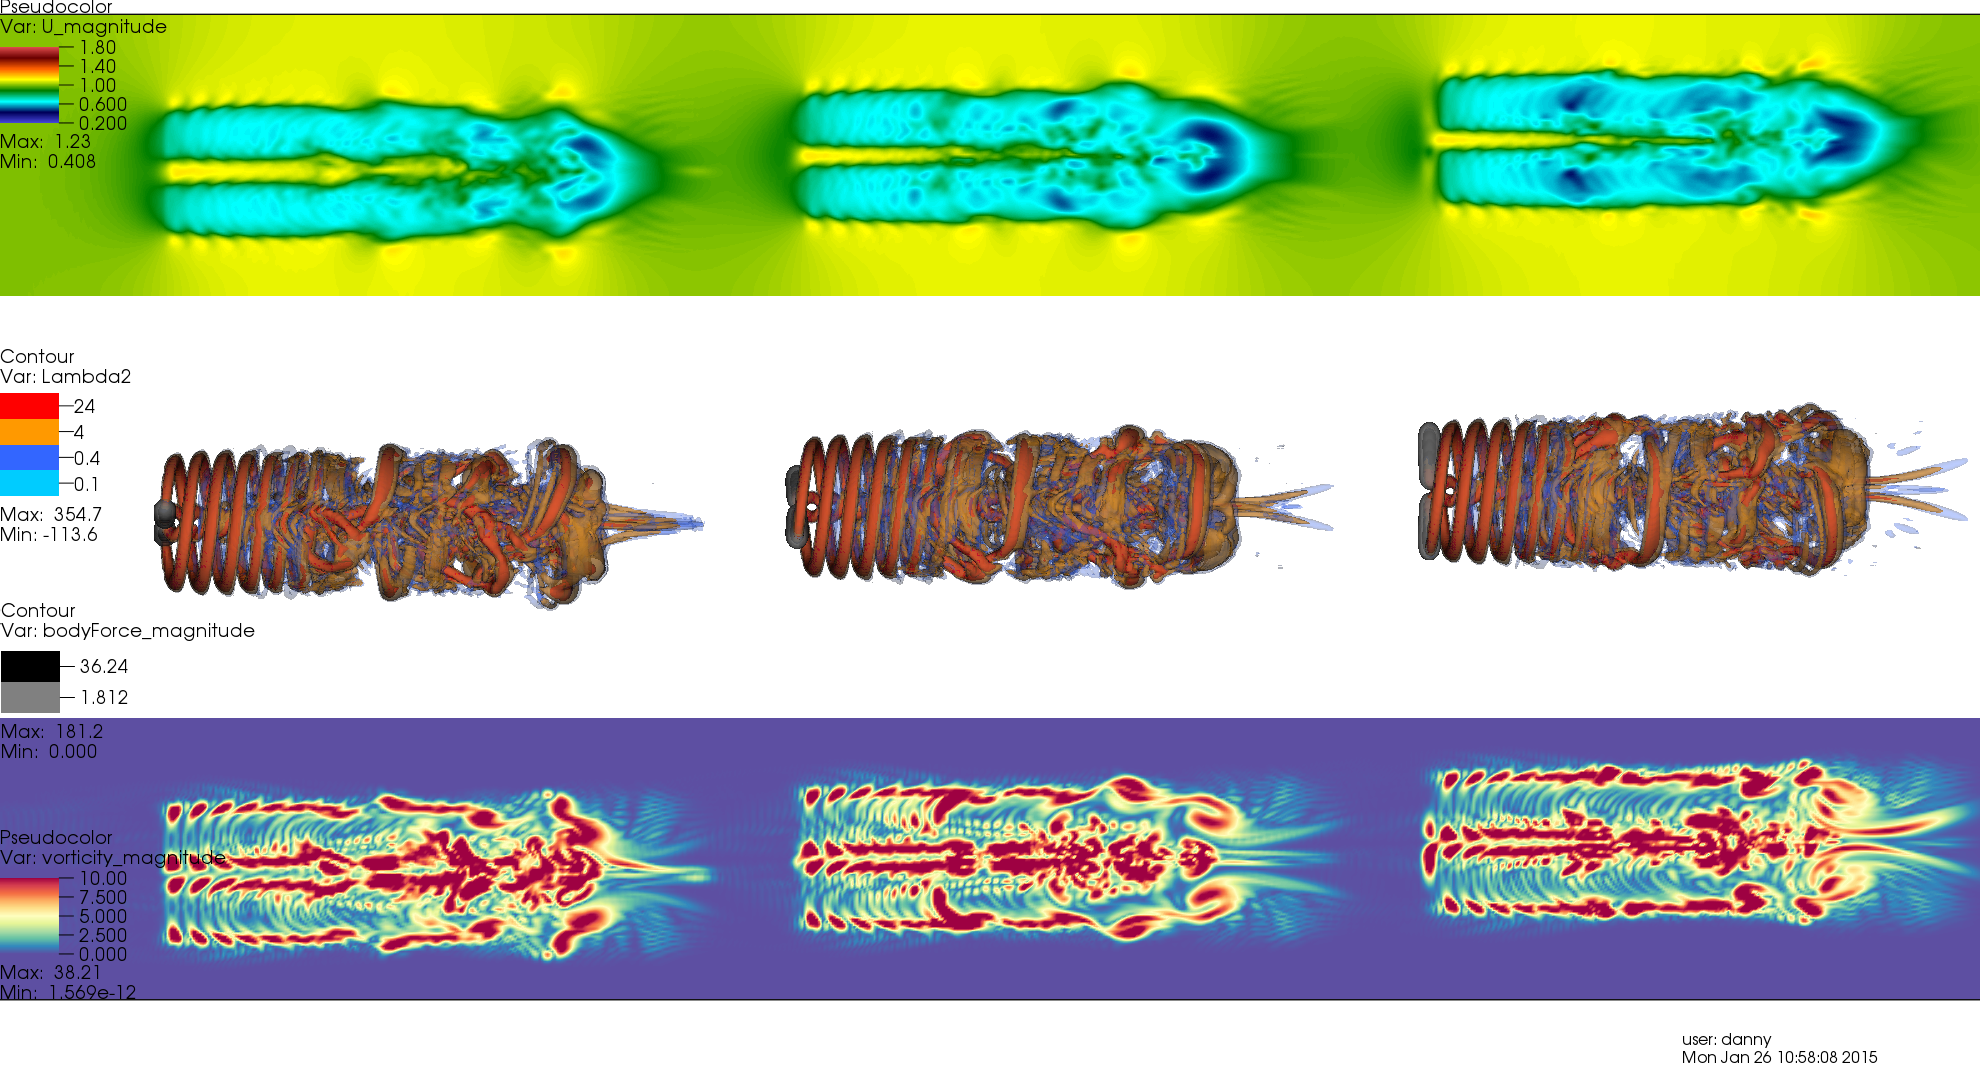
\includegraphics[width=1.05\textwidth]{figures/fastFlume__Turbines=3_TSR=6p2_Layout=offset_Mesh=fine.png}
		    \caption{\scriptsize{finer mesh 1047x113x90, dx = 0.00885 m}}
		\end{figure}

	\end{frame}

% 	\begin{frame}{again, at higher resolution}

% This time improved balance between mesh spacing with actuator discretization and body force spreading

% \tiny (but simulation time did not run as long yet)

% 		\begin{figure}[p]
% 		    \centering
%     		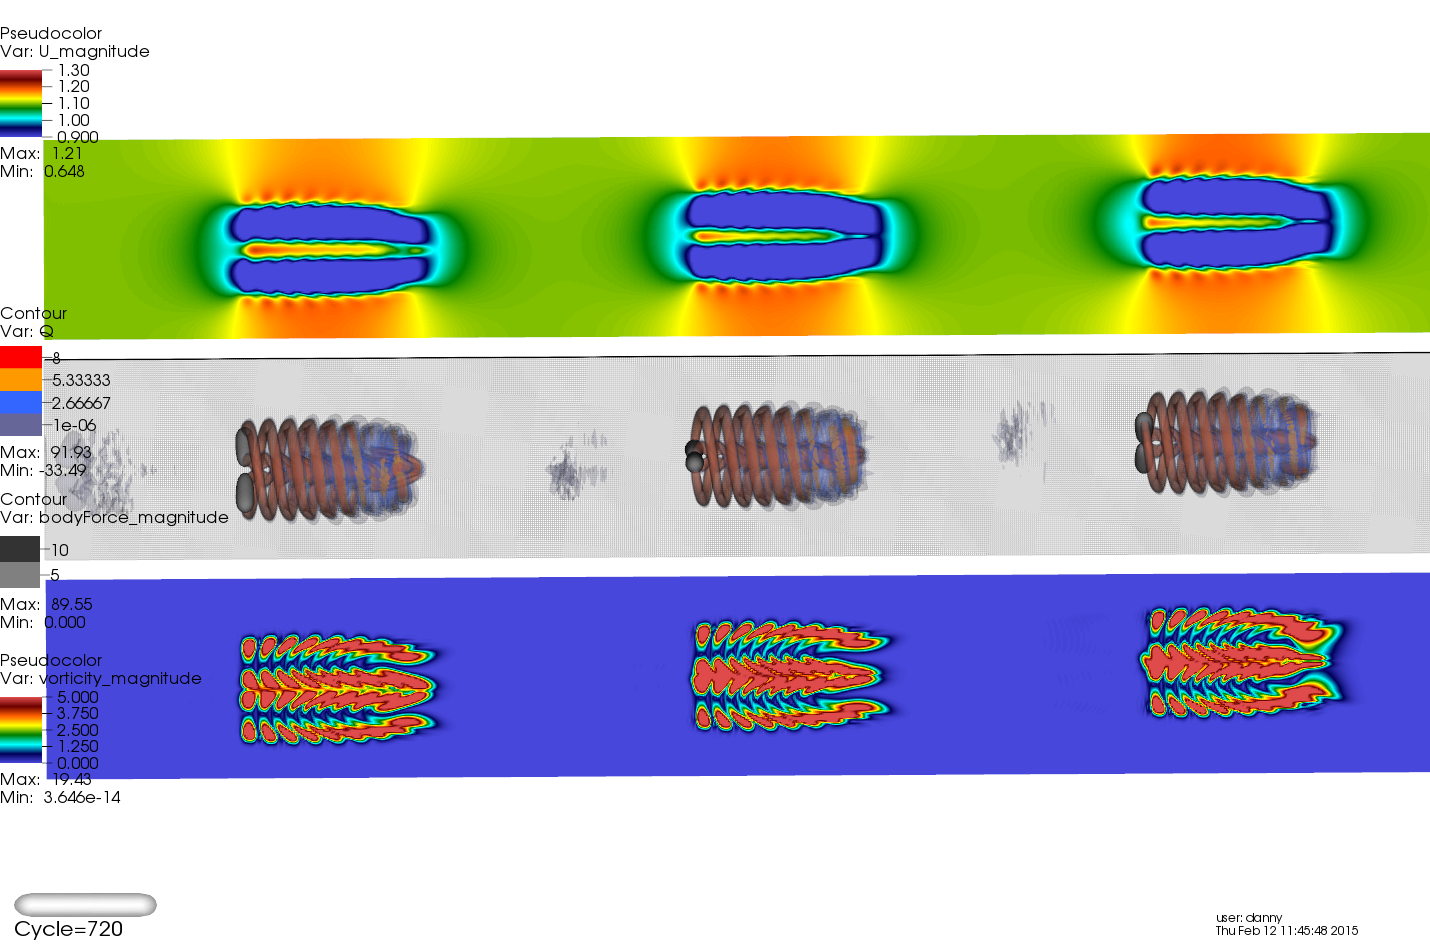
\includegraphics[width=0.8\textwidth]{figures/fastFlume__lab-scale-mesh=TunedFine.png}
% 		    \caption{\scriptsize{finer mesh 930x100x80, dx = 0.01 m}}
% 		\end{figure}

% 	\end{frame}

\subsection{analysis}
	
	\begin{frame}{}
		
		\vspace{-20pt}

		\begin{figure}[p]
		    \centering
		    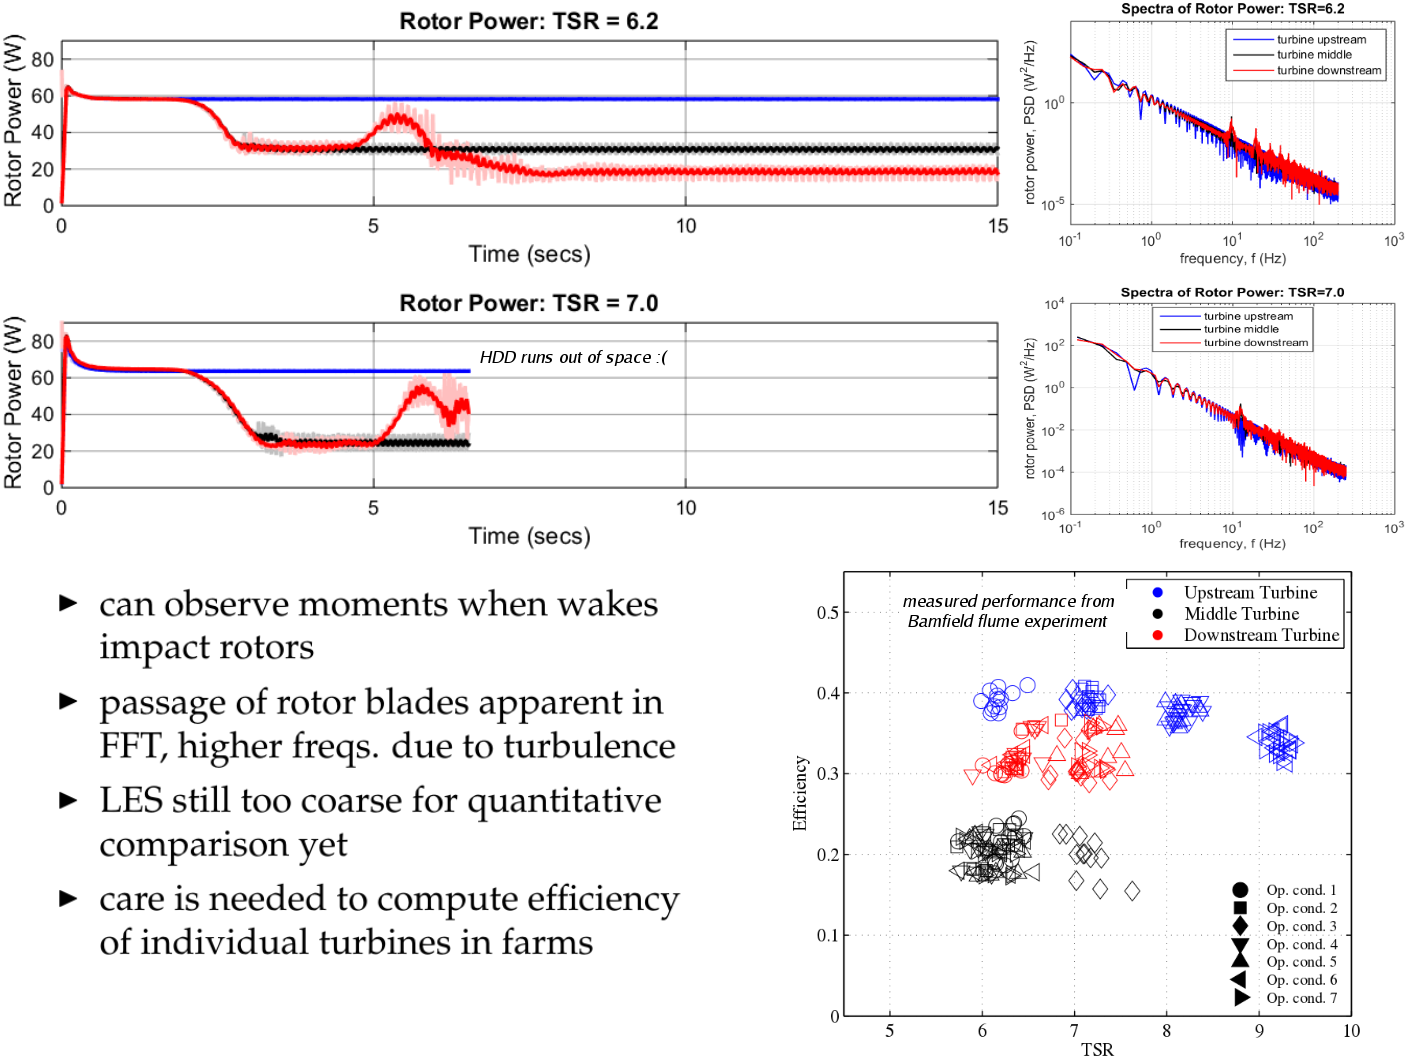
\includegraphics[width=1.08\textwidth]{figures/Analysis_Slide.png}
		\end{figure}

	\end{frame}

%%%%%%%%%%%%%%%%%%%%%%%%%%%%%%%%%%%%%%%%%%%%%%%%%%%%%%
%%%%%%%%%%%%%%%%%%%%%%%%%%%%%%%%%%%%%%%%%%%%%%%%%%%%%%
%%%%%%%%%%%%%%%%%%%%%%%%%%%%%%%%%%%%%%%%%%%%%%%%%%%%%%
%%%%%%%%%%%%%%%%%%%%%%%%%%%%%%%%%%%%%%%%%%%%%%%%%%%%%%
%%%%%%%%%%%%%%%%%%%%%%%%%%%%%%%%%%%%%%%%%%%%%%%%%%%%%%
%%%%%%%%%%%%%%%%%%%%%%%%%%%%%%%%%%%%%%%%%%%%%%%%%%%%%%
%%%%%%%%%%%%%%%%%%%%%%%%%%%%%%%%%%%%%%%%%%%%%%%%%%%%%%
%%%%%%%%%%%%%%%%%%%%%%%%%%%%%%%%%%%%%%%%%%%%%%%%%%%%%%
%%%%%%%%%%%%%%%%%%%%%%%%%%%%%%%%%%%%%%%%%%%%%%%%%%%%%%
%%%%%%%%%%%%%%%%%%%%%%%%%%%%%%%%%%%%%%%%%%%%%%%%%%%%%%
\section{\scshape Simulation Full Scale}

\subsection{dual rotor}

	\begin{frame}{DOE Reference Model 1 Tidal Turbine}
		
		\begin{columns}
		    
		    \begin{column}{0.6\textwidth}
		        \begin{figure}[p]
				    \centering
				    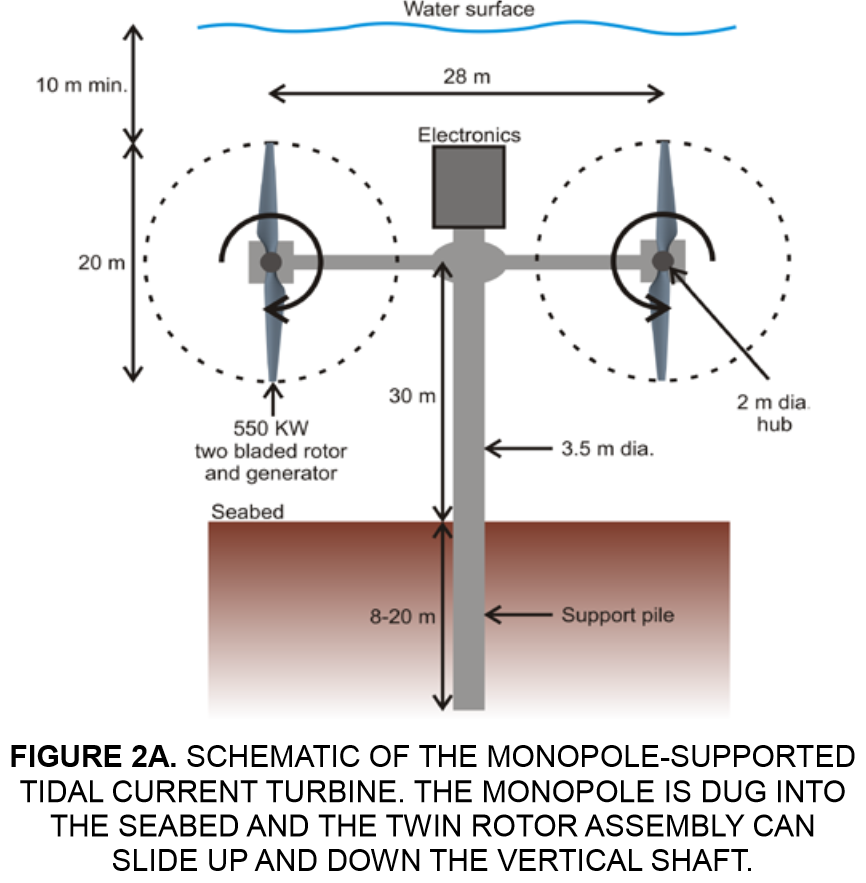
\includegraphics[width=0.8\textwidth]{figures/DOE-Reference-Model-1-Full-Scale-dual-rotor.PNG}
				    \caption{\scriptsize{Reference Model 1 Tidal Turbine}}
				\end{figure}

		    \end{column}
		    
		    \begin{column}{0.6\textwidth}
		        \begin{figure}[p]
				    \centering
				    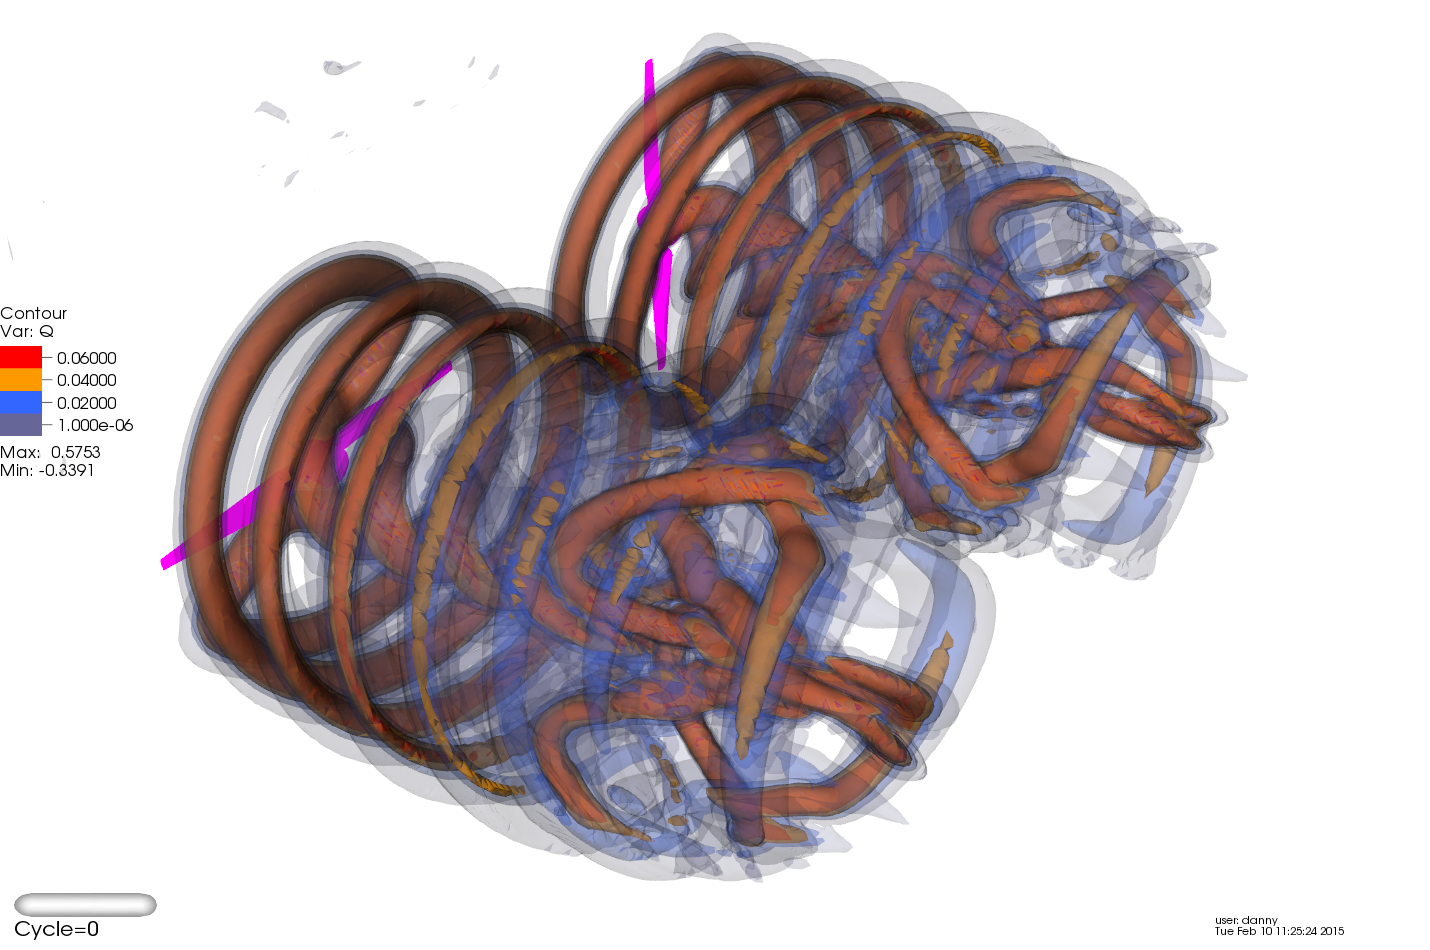
\includegraphics[width=0.8\textwidth]{figures/fastFlume__dual-rotor-mesh=TunedMedium.png}
				    \caption{\scriptsize{mesh 350x200x125, dx = 0.4 m}}
				\end{figure}

		    \end{column}

		\end{columns}

	\end{frame}

	\begin{frame}{}

		\begin{figure}[p]
		    \centering
    		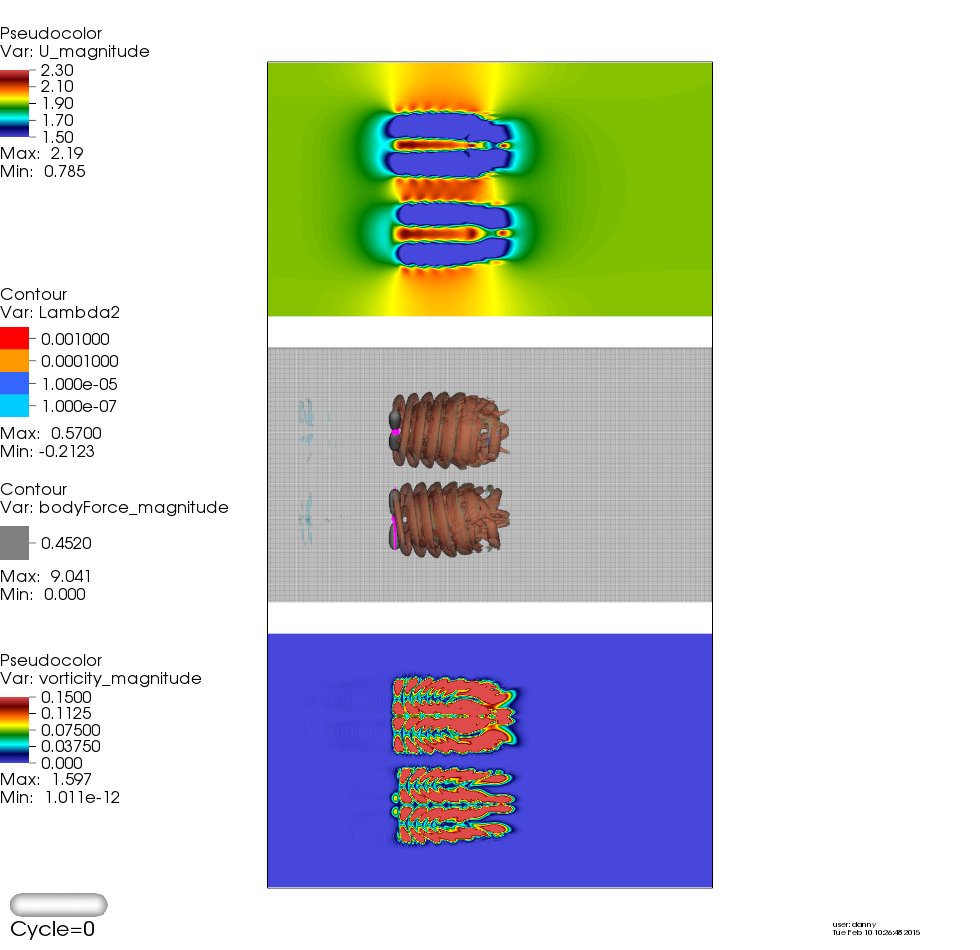
\includegraphics[width=0.8\textwidth]{figures/fastFlume__dual-rotor-mesh=medium-3vars.png}
		    \caption{\scriptsize{mesh 350x200x125, dx = 0.4 m}}
		\end{figure}

	\end{frame}

\subsection{analysis}
	
	\begin{frame}{}
		
		\vspace{-20pt}

		\begin{figure}[p]
		    \centering
		    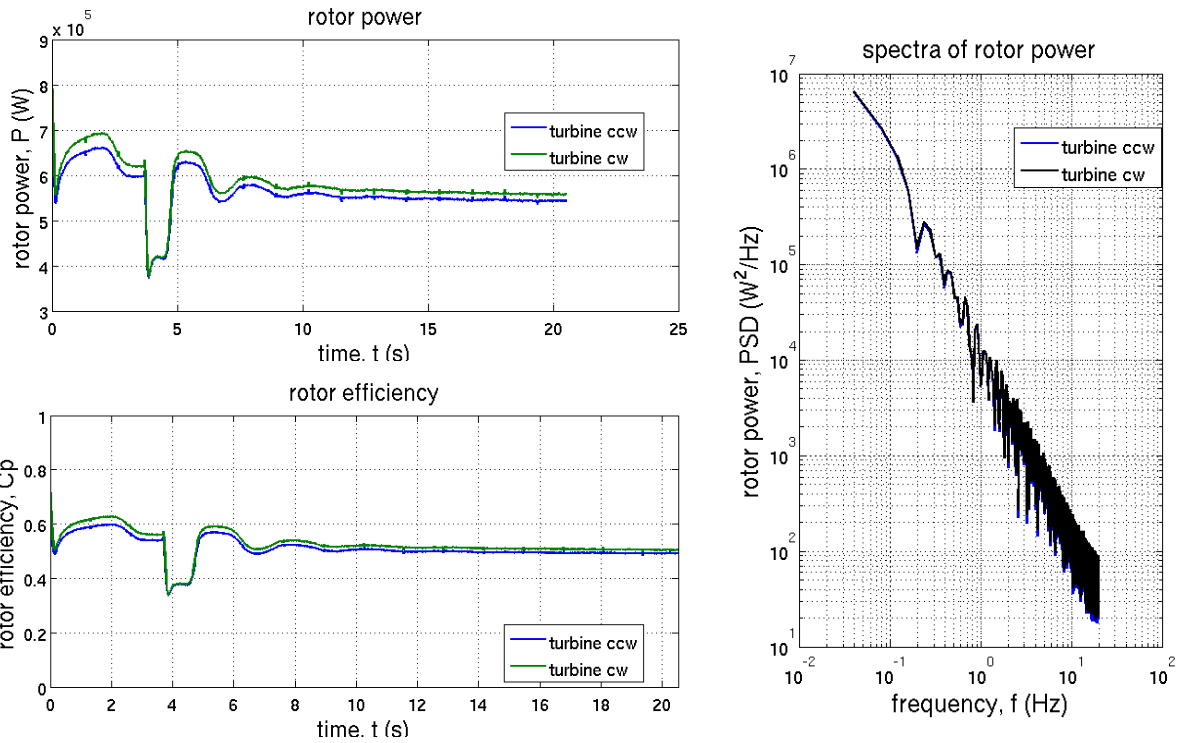
\includegraphics[width=1.08\textwidth]{figures/fastFlume__dual-rotor-mesh=TunedMedium-Analysis.png}
		\end{figure}

	\end{frame}

%%%%%%%%%%%%%%%%%%%%%%%%%%%%%%%%%%%%%%%%%%%%%%%%%%%%%%
%%%%%%%%%%%%%%%%%%%%%%%%%%%%%%%%%%%%%%%%%%%%%%%%%%%%%%
%%%%%%%%%%%%%%%%%%%%%%%%%%%%%%%%%%%%%%%%%%%%%%%%%%%%%%
%%%%%%%%%%%%%%%%%%%%%%%%%%%%%%%%%%%%%%%%%%%%%%%%%%%%%%
%%%%%%%%%%%%%%%%%%%%%%%%%%%%%%%%%%%%%%%%%%%%%%%%%%%%%%
%%%%%%%%%%%%%%%%%%%%%%%%%%%%%%%%%%%%%%%%%%%%%%%%%%%%%%
%%%%%%%%%%%%%%%%%%%%%%%%%%%%%%%%%%%%%%%%%%%%%%%%%%%%%%
%%%%%%%%%%%%%%%%%%%%%%%%%%%%%%%%%%%%%%%%%%%%%%%%%%%%%%
%%%%%%%%%%%%%%%%%%%%%%%%%%%%%%%%%%%%%%%%%%%%%%%%%%%%%%
%%%%%%%%%%%%%%%%%%%%%%%%%%%%%%%%%%%%%%%%%%%%%%%%%%%%%%

\section{\scshape Future Work}

\subsection{Future Work}

	\begin{frame}{Future Work}

		\begin{itemize}
			\item \footnotesize Code and Computers
				\begin{itemize}
					\item \footnotesize prototype simulations for running on more powerful hardware
					\item shared memory, distributed memory, co-processors
					\item want to understand resolution required to resolve wakes and turbine performance accurately
					\item based upon free and opensource software					
				\end{itemize}

			\item \footnotesize Ambient Turbulence
				\begin{itemize}
					\item \footnotesize turbulent structures within ambient flow can cause loading events with significance comparable to when turbines operate in upstream wakes
					\item boundary data on inlet planes generated from either precursor LES or synthetic turbulence methods (e.g. pyTurbSim)
				\end{itemize}

			\item \footnotesize Control Strategies
				\begin{itemize}
					\item \footnotesize dynamical model of rotor drivertrain to allow variable TSR as response to fluctuations in rotor torque
					\item rotor speed and pitch control for "in-water" dynamometer testing
				\end{itemize}
		\end{itemize}
	
	\end{frame}

%%%%%%%%%%%%%%%%%%%%%%%%%%%%%%%%%%%%%%%%%%%%%%%%%%%%%%
%%%%%%%%%%%%%%%%%%%%%%%%%%%%%%%%%%%%%%%%%%%%%%%%%%%%%%
%%%%%%%%%%%%%%%%%%%%%%%%%%%%%%%%%%%%%%%%%%%%%%%%%%%%%%
%%%%%%%%%%%%%%%%%%%%%%%%%%%%%%%%%%%%%%%%%%%%%%%%%%%%%%
%%%%%%%%%%%%%%%%%%%%%%%%%%%%%%%%%%%%%%%%%%%%%%%%%%%%%%
%%%%%%%%%%%%%%%%%%%%%%%%%%%%%%%%%%%%%%%%%%%%%%%%%%%%%%
%%%%%%%%%%%%%%%%%%%%%%%%%%%%%%%%%%%%%%%%%%%%%%%%%%%%%%
%%%%%%%%%%%%%%%%%%%%%%%%%%%%%%%%%%%%%%%%%%%%%%%%%%%%%%
%%%%%%%%%%%%%%%%%%%%%%%%%%%%%%%%%%%%%%%%%%%%%%%%%%%%%%
%%%%%%%%%%%%%%%%%%%%%%%%%%%%%%%%%%%%%%%%%%%%%%%%%%%%%%
\section{\scshape Validation}

\subsection{RANS-experiment-setup}
	
	\begin{frame}{}

		\scriptsize Simulations were performed with Reynolds Averaged Navier-Stokes (RANS) methods 
		to resolve geometry of blades and nacelle. Turbine wakes measured using
		particle image velocimetry (PIV) and acoustic Doppler velocimetry (ADV), and efficiency derived from
		torque and rotational speed measurements. 
		% \customfootcite{Javaherchi_a}
		% \customfootcite{Stelzenmuller_a}
		% \customfootcite{Javaherchi_b}
		\footfullcite{Javaherchi_a}
		\footfullcite{Stelzenmuller_a}
		\footfullcite{Javaherchi_b}

		\vspace{-5pt}

		\begin{figure}[p]
		    \centering
		    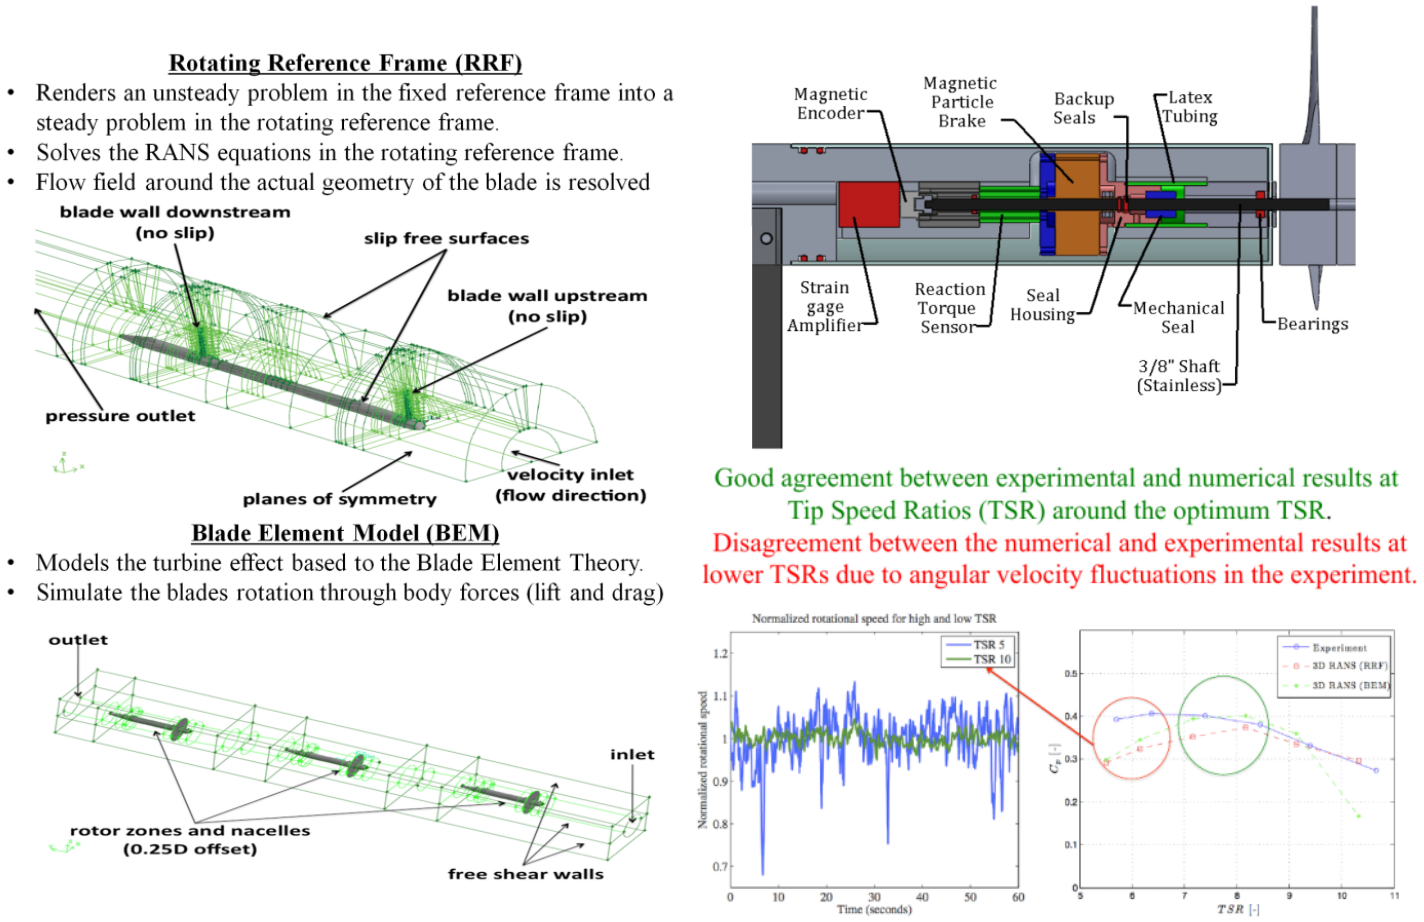
\includegraphics[width=0.75\textwidth]{figures/validation-RANS-experiment-setup.png}
		\end{figure}

	\end{frame}


\subsection{Single Turbine}
	
	\begin{frame}{}

		\begin{figure}[p]
		    \centering
		    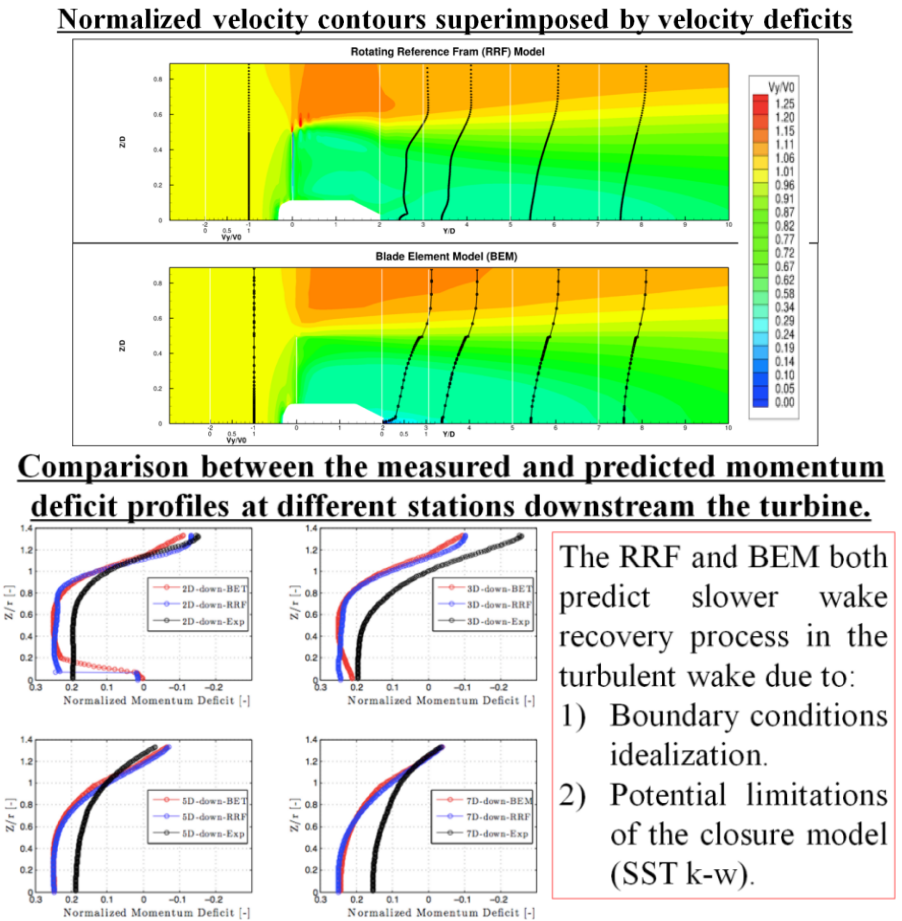
\includegraphics[width=0.75\textwidth]{figures/validation-RANS-experiment_single-turbine_performance-and-wake-1.png}
		\end{figure}

	\end{frame}

\subsection{Turbine Array}
	
	\begin{frame}{}

		\begin{figure}[p]
		    \centering
		    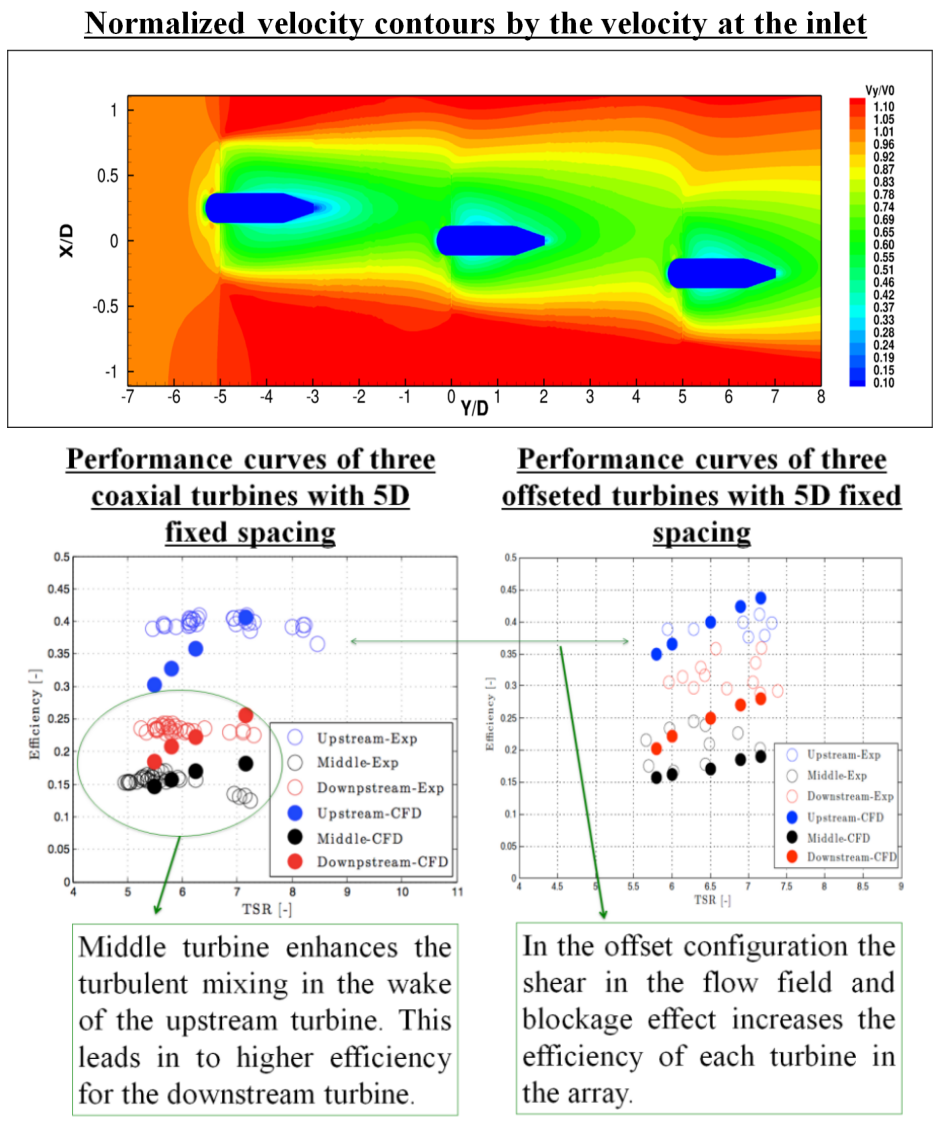
\includegraphics[width=0.65\textwidth]{figures/validation-RANS-experiment_turbine-array_performance-and-wake-1.png}
		\end{figure}

	\end{frame}

\subsection{to-do}
	
	\begin{frame}{}

		ongoing work: tabulate output from LES to overlay with RANS and experiments

	\end{frame}

%%%%%%%%%%%%%%%%%%%%%%%%%%%%%%%%%%%%%%%%%%%%%%%%%%%%%%
%%%%%%%%%%%%%%%%%%%%%%%%%%%%%%%%%%%%%%%%%%%%%%%%%%%%%%
%%%%%%%%%%%%%%%%%%%%%%%%%%%%%%%%%%%%%%%%%%%%%%%%%%%%%%
%%%%%%%%%%%%%%%%%%%%%%%%%%%%%%%%%%%%%%%%%%%%%%%%%%%%%%
%%%%%%%%%%%%%%%%%%%%%%%%%%%%%%%%%%%%%%%%%%%%%%%%%%%%%%
%%%%%%%%%%%%%%%%%%%%%%%%%%%%%%%%%%%%%%%%%%%%%%%%%%%%%%
%%%%%%%%%%%%%%%%%%%%%%%%%%%%%%%%%%%%%%%%%%%%%%%%%%%%%%
%%%%%%%%%%%%%%%%%%%%%%%%%%%%%%%%%%%%%%%%%%%%%%%%%%%%%%
%%%%%%%%%%%%%%%%%%%%%%%%%%%%%%%%%%%%%%%%%%%%%%%%%%%%%%
%%%%%%%%%%%%%%%%%%%%%%%%%%%%%%%%%%%%%%%%%%%%%%%%%%%%%%
\section{\scshape Outro}

\subsection{}
	\begin{frame}{}
		Thanks to SOWFA developers! Thanks to everybody involved with 
		modeling and validation of DOE Reference Model turbines!

		\printbibliography[heading=none]

	\end{frame}

%%%%%%%%%%%%%%%%%%%%%%%%%%%%%%%%%%%%%%%%%%%%%%%%%%%%%%
%%%%%%%%%%%%%%%%%%%%%%%%%%%%%%%%%%%%%%%%%%%%%%%%%%%%%%
%%%%%%%%%%%%%%%%%%%%%%%%%%%%%%%%%%%%%%%%%%%%%%%%%%%%%%
%%%%%%%%%%%%%%%%%%%%%%%%%%%%%%%%%%%%%%%%%%%%%%%%%%%%%%
%%%%%%%%%%%%%%%%%%%%%%%%%%%%%%%%%%%%%%%%%%%%%%%%%%%%%%
%%%%%%%%%%%%%%%%%%%%%%%%%%%%%%%%%%%%%%%%%%%%%%%%%%%%%%
%%%%%%%%%%%%%%%%%%%%%%%%%%%%%%%%%%%%%%%%%%%%%%%%%%%%%%
%%%%%%%%%%%%%%%%%%%%%%%%%%%%%%%%%%%%%%%%%%%%%%%%%%%%%%
%%%%%%%%%%%%%%%%%%%%%%%%%%%%%%%%%%%%%%%%%%%%%%%%%%%%%%
%%%%%%%%%%%%%%%%%%%%%%%%%%%%%%%%%%%%%%%%%%%%%%%%%%%%%%
\end{document}